\title{Shift Registers}
\begin{document}
\section{Types of Shift Registers}

\begin{frame}{Shift register}
  \begin{definition}
    A \alert{shift register} is an n-bit register that shifts its data by one bit each clock tick.
  \end{definition}
  \begin{itemize}
    \item Shift registers are useful in signal processing applications.
    \item Most microprocessors provide left and right shift assembly instructions.
  \end{itemize}
  What is useful about left and right shift assembly instructions?
\end{frame}

\subsection{Shift Register Structure}

Left and right shift operations divide and multiply by 2, respectively.

\begin{frame}{Serial-in, serial-out shift register}
  \begin{center}
    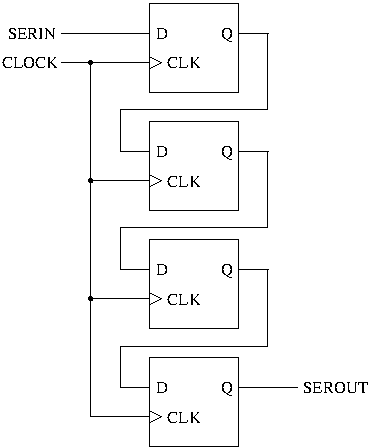
\includegraphics[scale=0.9]{SerialInSerialOutShiftRegister}
  \end{center}
\end{frame}

\begin{frame}{Serial-in, Parallel-out shift register}
  \begin{center}
    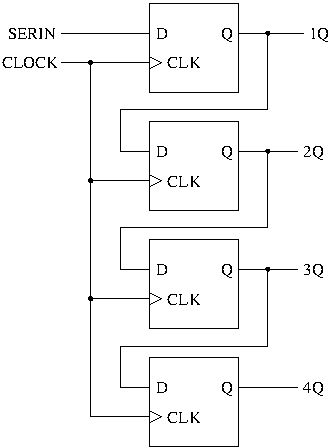
\includegraphics[scale=0.9]{SerialInParallelOutShiftRegister}
  \end{center}
\end{frame}

\begin{frame}{Parallel-in, Serial-out shift register}
  \begin{center}
    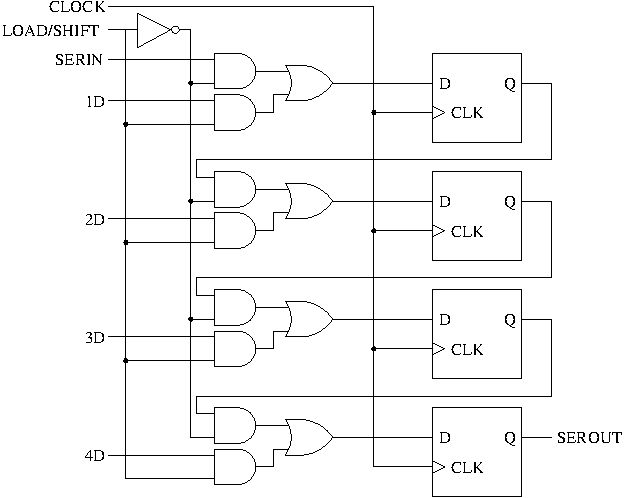
\includegraphics[scale=0.8]{ParallelInSerialOutShiftRegister}
  \end{center}
\end{frame}

\begin{frame}{Parallel-in, Parallel-out shift register}
  \begin{center}
    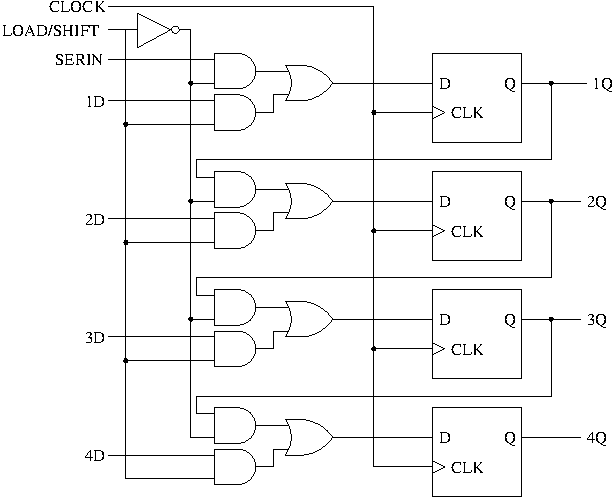
\includegraphics[scale=0.8]{ParallelInParallelOutShiftRegister}
  \end{center}
\end{frame}

\subsection{MSI Shift Register}

\begin{frame}{74x194 shift register}
  \begin{columns}
    \begin{column}{3cm}
      \begin{center}
        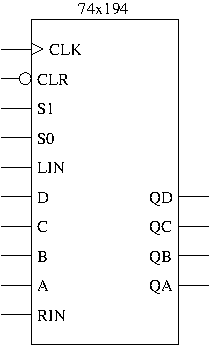
\includegraphics[scale=0.8]{74x194Schematic}
      \end{center}
    \end{column}
      \begin{column}{9cm}
        \begin{itemize}
          \item The other shift registers were \alert{unidirectional}.
          \item The 74x194 is \alert{bidirectional}.
        \end{itemize}
        \begin{center}
          \begin{tabular}{l|cc|cccc}
            \textbf{Function} & \textbf{S1} & \textbf{S0} & \textbf{QA*} & \textbf{QB*} & \textbf{QC*} & \textbf{QD*} \\
            \hline
            Hold & 0 & 0 & QA & QB & QC & QD \\
            Shift right & 0 & 1 & RIN & QA & QB & QC \\
            Shift left & 1 & 0 & QB & QC & QD & LIN \\
            Load & 1 & 1 & Q & Q & Q & Q \\
          \end{tabular}
        \end{center}
      \end{column}
  \end{columns}
\end{frame}

\begin{frame}{Design exercise}
  \begin{block}{Serious Problem}
    You want to watch the Lions game on TV, but those TV commentators are so wrong, you need to listen to the game using the Lions radio broadcast.  The TV broadcast is a bit delayed, so you hear what happens before you see it.
  \end{block}
  Design a digital circuit to delay the radio broadcast a variable amount so you can adjust the delay to synchronize it with the TV.
  \begin{itemize}
    \item You have an analog-to-digital converter that changes the analog radio broadcast into a bit stream.
    \item You like wise have a digital-to-analog convert that changes the bit stream back to an analog signal for your speakers.
    \item You have a dial that provides one of eight three bit outputs (000 - 111) depending on the dial position.
  \end{itemize}
\end{frame}

Please use a block diagram to describe your design.
\begin{center}
  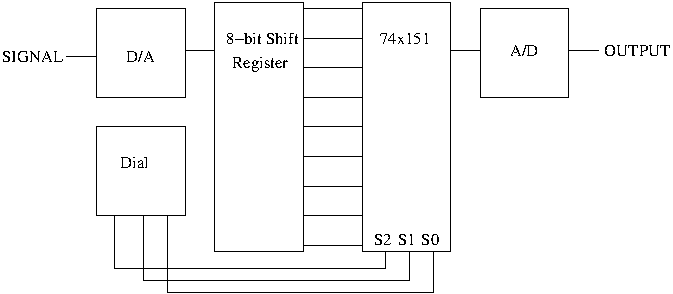
\includegraphics{SignalDelay}
\end{center}

\section{Shift Register Counters}

\begin{frame}{A counter that doesn't count}
  Often we may need to count something that doesn't occur in ascending or descending numeric order.
  \begin{definition}
    A \alert{shift-register counter} will count (or more specifically iterate) a fixed set of states in a cyclic manner.
  \end{definition}
  \begin{itemize}
    \item If we require a cyclic state machine, we can design the excitation and output logic to work with a certin shift-register counter sequence.
    \item The original Press Your Luck board worked like this.
  \end{itemize}
\end{frame}

\subsection{Ring Counters}

\begin{frame}{Ring counter}
  \begin{center}
    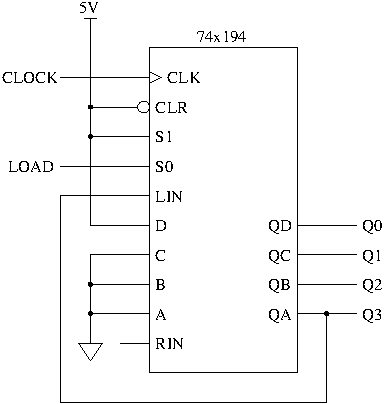
\includegraphics[scale=0.9]{74x194RingCounterSchematic}
  \end{center}
  What is a possible problem with this design?
\end{frame}

Write the state table for this counter.

\begin{frame}{A safer ring counter}
  \begin{center}
    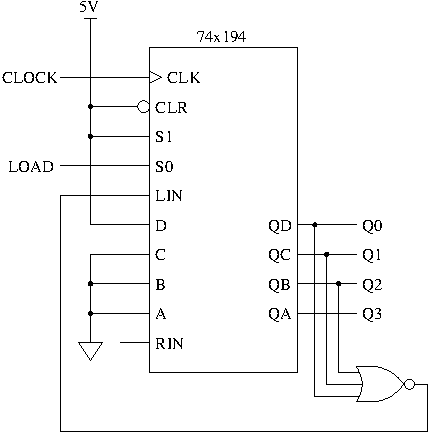
\includegraphics[scale=0.9]{74x194RingCounterCorrectingSchematic}
  \end{center}
\end{frame}

\begin{frame}{Unused states}
  In any state machine design, we must consider unsused states.
  \begin{itemize}
    \item Does the state machine have unused states?
    \item What is the chance one of these unused states will occur?
      \begin{itemize}
        \item Initialization
        \item Noise
      \end{itemize}
    \item Does each unused state return to a used state?
    \item Do we need to create special combinational logic to accomplish this?
  \end{itemize}
\end{frame}

\subsection{Johnson Counters}

\begin{frame}{Counter analysis}
  Let's analyze this counter.  How can we describe its output?
  \begin{center}
    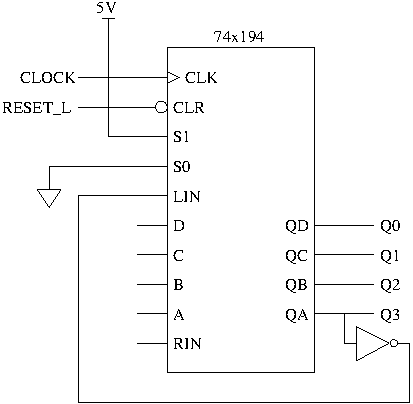
\includegraphics[scale=0.9]{74x194JohnsonCounterSchematic}
  \end{center}
\end{frame}
\end{document}
